%
% FDY TEMPLATE for ANUAL REPORT
% ===================================================================
% Reviewer 1: ...
% Reviewer 2: ...
%===================================================================
\NeedsTeXFormat{LaTeX2e}
\documentclass[11pt,twoside,a4paper]{fdyartcl}
\usepackage[utf8]{inputenc}
\usepackage[T1]{fontenc}
\usepackage[ngerman,english]{babel} % selectlanguage wird nur dann gebraucht, wenn
                                    % mehrere Sprachen-packages verwendet werden,
                                    % das zuletzt angegebene package ist die aktive
                                    % Sprache, mit \selectlanguage kann umgeschaltet
                                    % werden
\usepackage[intoc]{nomencl} % zur Erstellung einer Nomenklatur
                                   % Die Option [intoc] sorgt dafuer,
                                   % dass die Nomenklatur im
                                   % Inhaltsverzeichnis eingetragen
                                   % wird. Aufruf mit:
                                   % makeindex Diss.nlo -s nomencl.ist -o Diss.nls
\usepackage{longtable}  % fuer tabellen, die evtl ueber Seiten
                        % umgebrochen werden muessen
\usepackage{graphicx}   % Stellt \includegraphics zur Verfuegung
\usepackage{parskip}    % Setzt parindent auf null und parskip auf
                        % einen angemessenen Wert
\usepackage{calc}       % Erlaubt, verschiedene Masse zu addieren
                        % z.B 1cm+2pt
\usepackage[a4paper,twoside,outer=2.2cm,inner=3cm,top=1.5cm,bottom=2.7cm,includehead]{geometry}
                                        % erheblich verbesserte
                                        % Papieranassung
\usepackage{setspace}   % Stellt \singlespacing, \onehalfspacing und
                        % \doublespacig zur Verfuegung
                        % erlaubt ausserdem die Verwendung der
                        % Umgebung \begin{spacing}{2.3}
\setstretch{1.05}       % minimal vergroesserter Zeilenabstand
\usepackage{amsmath}    % Stellt verschiedene Mathematik Operatoren
                        % und Befehle bereit und verbessert die
                        % Darstellung von Gleichungen ermoeglicht
                        % ausserdem die Verwendung von \boldsymbol
                        % fuer z.B. griechische Buchstaben
\usepackage{amsfonts}
\usepackage{amsthm}
\usepackage{harvard}    % neue citation Befehle und anderes Layout der
                        % Bibliographie
\usepackage{mathpazo}   % Aenderung der Standardschrift auf Palatino
\bibliographystyle{diss_harv_babel}
\input babelbst.tex     % sonst funktioniert das zweite \cite Kommando
                        % nicht, weil im harvardstyle \bbletal{}
                        % herausgeschrieben wird
%\usepackage{showkeys}   % Spaeter auskommentieren
\usepackage{upgreek}    % nicht-kursive grichische Buchstaben
\usepackage{fancyhdr}

\usepackage{ngerman}    %erlaubt auf allen Btriebssystemen die Eingabe der Umlaute als "a,"o,"u und "s mit dem Ergebnis
                        % ä,ö,ü und ß.(Gleiches gilt für Großbuchstaben)
\usepackage{listings}
\usepackage{subfig}
\usepackage{hyperref}

\graphicspath{{./Figures/}}%
% \input hyphen_dt.tex  % Spezielle Trennregeln fuer deutsche
                        % Woerter - gehoert in den Vorspann
\clubpenalty = 10000%
\widowpenalty = 10000%
\displaywidowpenalty =10000


%%%%%%%%%%%%%%%%%%%%%%%%%%%%%%%%%%%%%%%%%%%%%%%%%%%%%%%%%%%%%%%%%%%%%
%%%%%%%%%%%%%%%%%%%%%%%%%%%%%%%%%%%%%%%%%%%%%%%%%%%%%%%%%%%%%%%%%%%%%
% TITLE AND AUTHOR
%%%%%%%%%%%%%%%%%%%%%%%%%%%%%%%%%%%%%%%%%%%%%%%%%%%%%%%%%%%%%%%%%%%%%
%%%%%%%%%%%%%%%%%%%%%%%%%%%%%%%%%%%%%%%%%%%%%%%%%%%%%%%%%%%%%%%%%%%%%
\title{Guide for HHLR Cluster}
\author{Stephan Krämer-Eis, Björn Müller, revised by Dennis Krause, Markus Geisenhofer}
%%%%%%%%%%%%%%%%%%%%%%%%%%%%%%%%%%%%%%%%%%%%%%%%%%%%%%%%%%%%%%%%%%%%%
%%%%%%%%%%%%%%%%%%%%%%%%%%%%%%%%%%%%%%%%%%%%%%%%%%%%%%%%%%%%%%%%%%%%%
%%%%%%%%%%%%%%%%%%%%%%%%%%%%%%%%%%%%%%%%%%%%%%%%%%%%%%%%%%%%%%%%%%%%%

%%%%%%%%%%%%%%%%%%%%%%%%%%%%%%%%%%%%%%%%%%%%%%%%%%%%%%%%%%%%%%%%%%%%%
%%%%%%%%%%%%%%%%%%%%%%%%%%%%%%%%%%%%%%%%%%%%%%%%%%%%%%%%%%%%%%%%%%%%%
% Kopfzeile
\pagestyle{fancy}
\fancyhf{}
\renewcommand{\headrulewidth}{0pt}

%\fancyhead[CE]{\sffamily \normalsize \thepage \quad \hrulefill \quad \sffamily \normalsize Short Title of Your Report }
%\fancyhead[CO]{\sffamily \normalsize F. Kummer \quad \hrulefill \quad \sffamily \normalsize \thepage }
\fancyhead[CE]{\sffamily \small \thepage \quad \hrulefill \quad \sffamily \small Guide for HHLR Cluster }
\fancyhead[CO]{\sffamily \small FDY \quad \hrulefill \quad \sffamily \small \thepage }


%%%%%%%%%%%%%%%%%%%%%%%%%%%%%%%%%%%%%%%%%%%%%%%%%%%%%%%%%%%%%%%%%%%%%
%%%%%%%%%%%%%%%%%%%%%%%%%%%%%%%%%%%%%%%%%%%%%%%%%%%%%%%%%%%%%%%%%%%%%

% Angaben fuer die Nomenklatur
%\makenomenclature
%\renewcommand{\nomname}{Nomenklatur}
%\setlength{\nomitemsep}{-0.2\parsep}% Der Abstand zweier Eintraege in
                                    % der Nomeklatur betraegt

% Dieser Befehl stellt sicher, dass neue Kapitel auf rechten (ungeraden) Seiten beginnen
\newcommand{\clearemptydoublepage}%
{\newpage{\pagestyle{empty}\cleardoublepage}}
\newfont{\myrm}{cmr12 at 12 pt}
% FigureXYLabel - urspruenglich in defin.tex, von Prof.~Dr.-Ing.~M. Oberlack
% Urspruengliche Version umfasste 5 Parameter -  geaenderte 7 Parameter - Bauerbach
% 1 Figurename: \includegraphics[......
% 2 Beschriftung der x Achse
% 3 x-Beschriftung - Verruecken horizontal positiv nach links
% 4 x Beschriftung - Verruecken vertikal positiv nach unten
% 5 Beschriftung der y Achse
% 6 y-Beschriftung - Verruecken horizontal positiv nach links
% 7 y Beschriftung - Verruecken vertikal positiv nach oben
\newlength{\FigureHeight}
\newlength{\FigureHeightHalf}
\newcommand{\FigureXYLabel}[7]{%
\settoheight{\FigureHeight}{#1}%
\setlength{\FigureHeightHalf}{0.5\FigureHeight}%
\addtolength{\FigureHeightHalf}{#7}%
\raisebox{\FigureHeightHalf}{\makebox[0cm][r]{#5\makebox[#6]{}}}%
#1\\%
\vspace{#4}%
{\makebox{#2\makebox[#3]{}}}}
%
%%%%%%%%%%%%%%%%%%%%%%%%%%%%%%%%%%%%%%%%%%%%%%%%%%%%%%%%%%%%%%%%%%%%%
%\addtokomafont{sectioning}{\rmfamily}
%\addtokomafont{section}{\normalsize}
%\addtokomafont{subsection}{\normalsize}

%\usepackage{sectsty}
%\sectionfont{ \parskip=0mm \vspace*{-5mm} }
%\subsectionfont{ \parskip=0pt \vspace*{-1mm} \centering \normalfont \normalsize \itshape}
%\paragraphfont{ \normalfont \itshape }





%       DOKUMENT
\begin{document}

\pagenumbering{arabic} % Zurueckschalten auf arabische Ziffern, dabei wird der Zaehler auf 1 gesetzt

%%%%%%%%%%%%%%%%%%%%%%%%%%%%%%%%%%%%%%%%%%%%%%%%%%%%%%%%%%%%%%%%%%%%%%%%%%%%%%%%55
% Seitennummer der ersten Seite
\setcounter{page}{1} % must be an odd number
                       % muss eine ungerade Zahl sein
%%%%%%%%%%%%%%%%%%%%%%%%%%%%%%%%%%%%%%%%%%%%%%%%%%%%%%%%%%%%%%%%%%%%%%%%%%%%%%%%55
%%%%%%%%%%%%%%%%%%%%%%%%%%%%%%%%%%%%%%%%%%%%%%%%%%%%%%%%%%%%%%%%%%%%%%%%%%%%%%%%55
%%%%%%%%%%%%%%%%%%%%%%%%%%%%%%%%%%%%%%%%%%%%%%%%%%%%%%%%%%%%%%%%%%%%%%%%%%%%%%%%55

% Titelseite
% -------------------
\maketitle


\begin{abstract}
%\textbf{Abstract:}
This best practice guide gives an overview over the required steps to run BoSSS on the HHLR cluster. It gives some informations about the cluster itself and starts with a step by step tutorial how to install the necessary libraries on the cluster. Furthermore a commented batch script is given to run a BoSSS application on the compute nodes.
\end{abstract}




%==================== Hauptteil =====================================
%
\section{Notation}
\label{sec:notation}
\begin{description}
	\item[\$executable] The path to the BoSSS binary on your local machine which you want to  execute on the cluster
	\item[\$BoSSSDir] Local directory to your BoSSS repository
	\item[\$TuID] Your TU-ID
	\item[\$home] Your home directory on the cluster
	\item[\$executionDir] An arbitrary sub-directory of \verb|$home| to which the executables will be deployed
	\item[\$databaseDir] The location of a BoSSS database on the cluster (usually a sub-directory of \verb|$home|)
	\item[\$host] The host name of one of the login nodes of the cluster. Currently, you can select lcluster2.hrz.tu-darmstadt.de, lcluster3.hrz.tu-darmstadt.de or lcluster4.hrz.tu-darmstadt.de
\end{description}

\section{General information about the cluster}
\label{sec:information}

The HHLR Lichtenberg cluster consists of 780 compute nodes and 4 login nodes. The cluster is split into 4 sections: 
\begin{itemize}
	\item MPI, for MPI intensive applications
	\item MEM, for memory intensive applications
	\item ACC, for applications which are using accelerators, like GPU computations
	\item SMP, for computation and memory intensive applications (under construction!)
\end{itemize}
The compute nodes are subdivided into 19 islands: 17 island with each 32 nodes (512 cores), 1 island with 160 nodes (2560 cores) and 1 island with accelerator nodes (CUDA cores and Xeon Phi Coprocessors). For BoSSS applications the MPI section is most suitable, to which the 17 islands and the island with 160 nodes belong. Each of this nodes consists of 2 processors with 8 cores (in total 16 cores per node) and 32 GB memory.\\
The file system is divided into 3 sections:
\begin{itemize}
\item \verb|/home|: With your application for an account, you get your home directory which you can find under \verb|/home/$TuID|. This directory can be accessed from all nodes and has a daily backup of your data. The quota is limited to 15 GB. 
\item \verb|/work/local|: These are the local hard drives of the node and can only be accessed from the particular node. Attention: After a job has finished, all data will be erased! 
\item \verb|/work/scratch|:  This directory can be accessed from all nodes. With your application, there will be the folder \verb|/work/scratch/$TuID|. You have unlimited quota, but all data is erased after 30 days without any warning! 
\end{itemize}
%More information: \url{http://www.hhlr.tu-darmstadt.de/hhlr/index.de.jsp}


\section{Installation on the cluster}

The HHLR cluster provides the user with some preinstalled libraries, like \verb|openmpi| or \verb|matlab|. The command \verb|module available|  lists them all. To run a BoSSS application on the cluster the Linux C\# compiler \emph{mono} must be manually installed. Additionally the libraries \emph{ParMETIS} and \emph{HYPRE} are needed. \emph{ParMETIS} is used for partitioning the grid and distributed the cells to each core. \emph{HYPRE} is used to solve large linear systems. This library is needed if you use, e.g., implicit time-stepping schemes.\\
There are two ways to install the libraries:
\begin{itemize}
\item Download the latest version from the developers homepage and install them manually
\item Copy the binaries from the local BoSSS repository onto the cluster 
\end{itemize}
Up to now \emph{mono} and \emph{HYPRE} needs to be installed. Binaries for \emph{ParMETIS} can be found in the BoSSS repository.

\subsection{Connecting to the cluster}
\label{sec:putty}
In general, the \emph{ssh} protocol is used to access the cluster. An \emph{ssh} connection can be established by simply using the \emph{ssh} command on the console (see the following section), but more sophisticated tools exist that allow for a simpler configuration of advanced connection settings. On Windows machines, the program \emph{PuTTY} is used predominantly, and this tutorial will briefly demonstrate its usage in section \ref{sec:dbe}. It should be noted, however, that \emph{PuTTY} is nothing but a graphical wrapper around the plain \emph{ssh} which means that all options can be used on the console, too.


\subsection{Installing \emph{mono}}
\label{sec:mono}
This is a step-by-step guide to install \emph{mono} the cluster. In total it takes about 1 hour to finish the installation!
\begin{enumerate}
\item Go to the developers homepage \url{http://download.mono-project.com/sources/mono/} and copy the link of your desired mono version (\verb|$mono-link|). As of December 2017 mono-5.9.0.415 is tested and working.
\item Open a git bash and login on one of the four login nodes of the cluster, e.g 1
\begin{verbatim}
ssh $TuID@$host
\end{verbatim}
\item Create a new directory \verb|mono| in \verb|$home| and open it
\begin{verbatim}
mkdir mono
cd mono
\end{verbatim}
\item Download the \emph{mono} archive into the directory
\begin{verbatim}
wget $mono-link
\end{verbatim}
\item Open \emph{mono} archive
\begin{verbatim}
tar -xjf mono-x.x.x.tar.bz2
\end{verbatim}
\item open the created folder
\begin{verbatim}
cd mono-x.x.x
\end{verbatim}
\item before compilation, mono has to be configured, which requires \emph{cmake}. Prefix gives the directory for the binaries (these are two commands)
\begin{verbatim}
module load cmake
./configure --prefix=/home/$TuID/mono/mono-x.x.x_bin
\end{verbatim} 
\item After a successful configuration the compilation can be started
\begin{verbatim}
make
\end{verbatim}
It can happen that the compiler ask for additional prompts. Just type \verb|.| and return.
The whole compilation takes about 50-60 minutes!
\item to finish the installation prompt
\begin{verbatim}
make install
\end{verbatim} 
\item Finally \emph{mono} has to be added to the \verb|PATH| and \verb|LD_LIBRARY_PATH| variable. This can be done in the .bashrc file: Go back to your \verb|$home| directory and open the .bashrc with an editor, e.g. vi
\begin{verbatim}
cd ~
vi .bashrc
\end{verbatim}
add to following lines for the \verb|PATH| variable (press \emph{i} to insert text)
\begin{verbatim}
PATH=/home/$TuID/mono/mono-x.x.x_bin/bin:$PATH
export PATH
\end{verbatim}
and for the \verb|LD_LIBRARY_PATH| variable
\begin{verbatim}
LD_LIBRARY_PATH=/home/$TuID/mono/mono-x.x.x_bin/lib:$LD_LIBRARY_PATH
export LD_LIBRARY_PATH
\end{verbatim}
Press \emph{Esc} and type \emph{:wq} to save your latest changes and quit the application. Save the changes and reload .bashrc by prompting
\begin{verbatim}
source .bashrc
\end{verbatim}
\end{enumerate} 

\subsection{Installing \emph{HYPRE}}
Installing \emph{HYPRE} works similar to the installation routine of \emph{mono} (see section \ref{sec:mono}). Hence only the bash commands are given:
\begin{enumerate}
\item go to the developers homepage \url{http://computation.llnl.gov/casc/hypre/software.html} and copy the link of your desired hypre version (\verb|$hypre-link|). 
\item login on the cluster
\begin{verbatim}
ssh $TuID@$host
\end{verbatim}
\item 
\begin{verbatim}
mkdir hypre
cd hypre
\end{verbatim}
\item 
\begin{verbatim}
wget $hypre-link
\end{verbatim}
\item Note the different tar command
\begin{verbatim}
tar -xzf hypre-x.x.x.tar.gz
\end{verbatim}
\item 
\begin{verbatim}
cd hypre-x.x.x/src
\end{verbatim}
\item Note the additional command --enable-shared 
\begin{verbatim}
./configure --prefix=/home/$TuID/hypre/hypre-x.x.x_bin --enable-shared
\end{verbatim} 
\item 
\begin{verbatim}
make
\end{verbatim}
\item
\begin{verbatim}
make install
\end{verbatim} 
\item only the \emph{HYPRE} library is used thus only the \verb|LD_LIBRARY_PATH| variable has to be adjusted in .bashrc
\begin{verbatim}
cd ~
vi .bashrc
\end{verbatim}
and add
\begin{verbatim}
LD_LIBRARY_PATH=/home/$TuID/hypre/hypre-x.x.x_bin/lib:$LD_LIBRARY_PATH
export LD_LIBRARY_PATH
\end{verbatim}
save the changes and reload .bashrc by prompting
\begin{verbatim}
source .bashrc
\end{verbatim}
\end{enumerate} 

\subsection{Installing \emph{ParMETIS}}
BoSSS does not work with the latest version of \emph{ParMETIS}. Therefore an older version is needed. You can find the binary in the BoSSS repository. Note: You find \emph{ParMETIS} only in the GridOfTomorrow branch!
\begin{enumerate}
\item copy the \emph{ParMETIS} binary folder on the cluster
\begin{verbatim}
scp -r $BoSSSDir/public/src/ilPSP/layer_0/3rd_party/ParMETIS $TuID@$host:~/ParMETIS/
\end{verbatim}
\item login on the cluster
\begin{verbatim}
ssh $TuID@$host
\end{verbatim}
\item build \emph{ParMETIS} using the bash-script \emph{buildParMETIS.sh}
\begin{verbatim}
cd ~/ParMETIS
dos2unix buildParMETIS.sh
bash buildParMETIS.sh
\end{verbatim}
\item  add the \emph{ParMETIS} library to the \verb|LD_LIBRARY_PATH| variable in .bashrc
\begin{verbatim}
vi .bashrc
\end{verbatim}
and add
\begin{verbatim}
LD_LIBRARY_PATH=/home/$TuID/ParMETIS/:$LD_LIBRARY_PATH
export LD_LIBRARY_PATH
\end{verbatim}
\end{enumerate}
Note: \verb|export LD_LIBRARY_PATH| needs only to be called once after the last change of the \verb|LD_LIBRARY_PATH|.\\\\
\textit{Remark: If it does not compile it is easier to use the compiled binaries instead. You can find them in} \verb|\\dc1\bosss\binaries\hhlr\ParMETIS|
\subsection{Installing \emph{PARDISO V5}}
\begin{enumerate}
\item download the newest \emph{PARDISO} Version from the Website \emph{http://www.pardiso-project.org} or from \verb|\\scratch\kummer\pardiso.zip| and copy the \verb|.so|-file to \verb|\home\$TUID/PARDISO|
\item  add the \emph{PARDISO} library to the \verb|LD_LIBRARY_PATH| variable in .bashrc
\begin{verbatim}
vi .bashrc
\end{verbatim}
and add
\begin{verbatim}
LD_LIBRARY_PATH=/home/$TuID/PARDISO:$LD_LIBRARY_PATH
export LD_LIBRARY_PATH
\end{verbatim}
\item get a licence from the pardiso website
\item open PardisoSolver.cs of your version of BoSSS
\item change Version m\_Version = Version.MKL to Version m\_Version = Version.v5 and add your licence key in between the quotation marks as seen below
%\item add the following to your xml-file
%\begin{verbatim}
%	  <sparsesolver name="PARDISO-V5">
%	    <type>direct</type>
%	    <library>pardiso</library>
%	    <specific>
%	      <Version>v5</Version>
%	      <!-- username '$TUID', (Lichtenberg) no NODE-lock : -->
%	      <LicenseCode>PUT LICENCE CODE HERE</LicenseCode>
%	    </specific>
%	  </sparsesolver>
%\end{verbatim}
\end{enumerate}
\begin{figure}[htbp] % htb: preferred position of picture: here, top, bottom of page
	\begin{centering}
		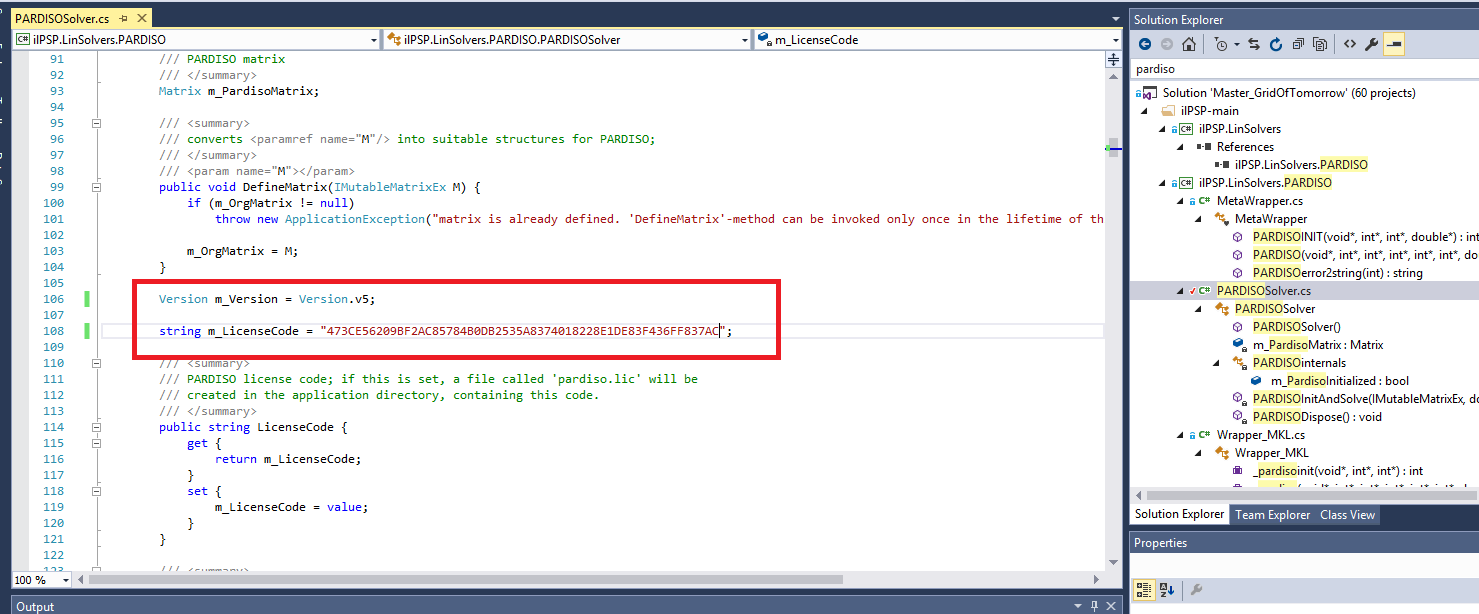
\includegraphics[width=0.9\textwidth]{Figures/pardiso_licence.png}\\
	\end{centering}
	\caption{Add your key to the Pardiso Solver}\label{fig:pardiso_licence}
\end{figure} %

\subsection{Installing \emph{MUMPS V5.0.2}}
In the following the compilation of MUMPS on the Lichtenberg cluster will be explained.
\begin{enumerate}
	\item Download MUMPS\_5.0.2 from the MUMPS website and unzip it.
	\item Copy the \textbf{Makefile.inc} into the main MUMPS folder and the \textbf{build\_shared} script to the \textit{/lib} directory. You can find both files in the underlying folder \textit{Lichtenberg} in the same directory as this document.
	\item Load modules \textbf{intel/2016u4} (2017 does not work) and one \textbf{openmpi/intel/2.0.1}.
	\item Execute the makefile by typing 'make'.
	\item If all went well there should be three libraries, naming libdmumps.a, libmumps\_common.a and libpord.a in your \textit{/lib} folder.
	\item Open the \textbf{build\_shared} and adjust the path to a folder in your home directory
	\item Execute the \textbf{build\_shared} by typing './build\_shared'. If you do not get permission to execute it, copy each line and run them separately.
	\item Modify your \textbf{.bashrc} and add the path to your libdmumps.so.	
\end{enumerate}
Now it should be possible to run the MUMPS solver on the Lichtenberg cluster in the same way you do on windows. 

The performance of MUMPS can possibly be increased by linking against Metis and Parmetis. At this stage there was a conflict between BoSSS, using Parmetis 3 and MUMPS, using Parmetis 4. As a reason the software Pord, which is distributed with MUMPS is being used for partitioning.

\subsection{Testing the libraries}
\label{sec:testing}
All necessary libraries are installed on the cluster. Now we can test them by running a small BoSSS application. As test problem, we choose the ipPoisson problem. In this particular case we run the problem directly on the login node, because it takes only a few seconds to compute. In general: Never run a computation on a login node! How to run a computational heavy application is explained later in section \ref{sec:WorkingHHLR}.

\textbf{Important note about the console application you use:} If you use \emph{git bash}, you should consider using another one (at least for this case). As \emph{git bash} is based on a console named \emph{mintty} which Windows recognizes as a normal program and not as a console application, there will be problems when entering your password for the Lichtenberg cluster, without going into too much detail. Alternatives are other console applications, such as \emph{cmd}, \emph{powershell} or \emph{ConEmu}. The last mentioned one is quite popular at FDY.

\begin{enumerate}
\item compile the ipPoisson project (in src/public/L4-applications/ipPoisson) on your local machine, e.g in Visual Studio
\item transfer the application and its dependencies to the cluster by using the \verb|bcl deploay-at| command (\verb|$executable| is for example\\
 \verb|/c/BoSSS/src/public/L4-application/ipPoisson/bin/Release/ipPoisson.exe|)
\begin{verbatim}
bcl deploy-at $executable sftp://$TuID@$host:~/ipPoisson
\end{verbatim}
\item \verb|bcl deploy-at| only copies the application but not a control file. Copy a suitable control file by using \verb|scp|
\begin{verbatim}
scp control-example.xml $TuID@$host:~/ipPoisson
\end{verbatim}
\item login on the cluster
\begin{verbatim}
ssh $TuID@$host
\end{verbatim}
\item before running the ipPoisson problem three additional libraries needs to be loaded: \verb|acml|, which includes the \verb|BLAS| library and \verb|openmpi|. For running \verb|acml|, the module \verb|gcc| is additionally needed.
\begin{verbatim}
module load acml
module load gcc
module load openmpi/gcc/1.6.6
\end{verbatim} 
\item now the program can be started
\begin{verbatim}
cd ipPoisson
mono ipPoisson.exe --control control-example.xml
\end{verbatim}
\item if everything is working, the program should be end with \verb|converged? true|. Then a parallel run on two cores can be tested:
\begin{verbatim}
mpiexec -n 2 mono ipPoisson.exe --control control-example.xml
\end{verbatim} 
\end{enumerate}
If both tests run, the installation of BoSSS on the HHLR cluster was successful.

\section{Setup and synchronization of the BoSSS database}
\label{sec:BoSSSdb}
For most of the BoSSS applications you need a database (db). Since you cannot use the graphical Database Explorer on the cluster, you need to synchronize your db on your local machine in order to evaluate your results.

\subsection{Setting up a database}
\label{sec:setup_db}
The easiest way to setup a database on the cluster is to generate it locally and then just copy it onto the cluster.
\begin{enumerate}
\item create locally a new folder for your db, e.g. \verb|c:\BoSSS_db|
\item open git bash and go to the folder, then prompt
\begin{verbatim}
bcl init-db
\end{verbatim}
\item now you have created a new db locally. By using \verb|scp| you can copy it to the cluster:
\begin{verbatim}
scp -r /c/BoSSS_db/ $TuID@$host:~/
\end{verbatim}
\end{enumerate}

\subsection{Synchronizing databases}
\label{sec:synchronize_db}
There are many ways to synchronize the db. An easy way is to use the tool \emph{WinSCP}. First you have to enter your login data, shown in figure \ref{fig:winscp_login}.
\begin{figure}[htbp] % htb: preferred position of picture: here, top, bottom of page
  \begin{centering}
  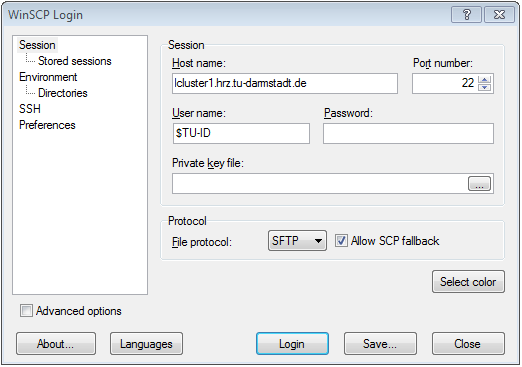
\includegraphics[width=0.9\textwidth]{Figures/winscp_login.png}\\
  \end{centering}
  \caption{WinSCP - Login data}\label{fig:winscp_login}
\end{figure} %
After logging in, you see on the left side your local file system and on the right side is your \verb|$home| directory on the cluster. Browse in both windows to the generated db (according to section \ref{sec:setup_db} this would be \verb|c:\BoSSS_db| on your local machine and \verb|/home/$TuID/BoSSS_db| on the cluster). \emph{WinSCP} has a build in synchronization tool, which is indicated with a red circle in figure \ref{fig:winscp_sync}.
\begin{figure}[htbp] % htb: preferred position of picture: here, top, bottom of page
  \begin{centering}
  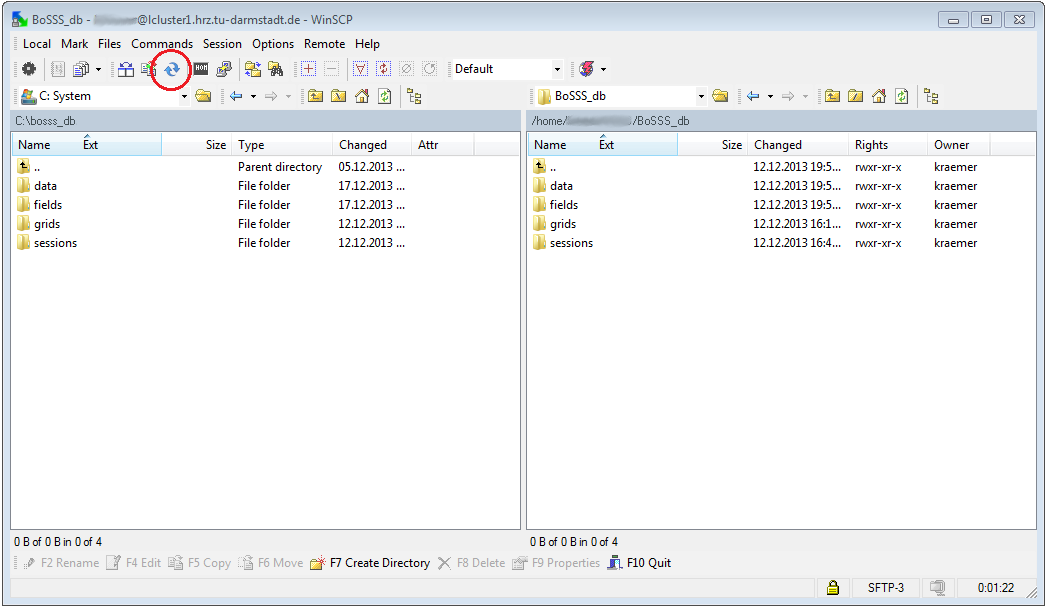
\includegraphics[width=0.9\textwidth]{Figures/winscp_sync.png}\\
  \end{centering}
  \caption{WinSCP - Synchronization}\label{fig:winscp_sync}
\end{figure} %
For the synchronization you have different options, e.g. from local to remote, from remote to local or in both directions.
You can also copy single files per drag and drop between both windows.

\subsection{Tips and Tricks}
\label{sec:tips}
\begin{itemize}
\item As mentioned in section \ref{sec:information} you have a quota of 15 GB in your home directory. If your planning big and/or many simulations, you might exceed this limit. Instead of using your \verb|$home| directory, you can use \verb|/work/scratch/$TuID| for your db. It has the advantage that you have nearly unlimited quota and \verb|/work/scratch| is a faster file system, i.e. less time is needed to save each timestep. But be careful: You have to take care of the data. On \verb|/work/scratch| data is deleted after 30 days without any warning!
\item If you have big databases and want them to synchronize only in one direction, e.g from the cluster on your local machine, it can take some time. Reason is that BoSSS saves every field in each timestep in a single file, hence you have lots of small files to copy. It can be faster to put the whole db in one archive and then just copy the archive to your local machine.
\end{itemize}


\section{Working on the HHLR Cluster}
\label{sec:WorkingHHLR}
As mentioned in Section \ref{sec:information} the cluster has 4 login nodes and 780 working nodes. The login nodes are only intended to access the cluster, to copy data and to prepare/submit jobs. Do not start any computation on the login nodes!
\subsection{Prepare a job}
The preparation for a job is similar like the first steps of testing the libraries in section \ref{sec:testing}:
\begin{enumerate}
\item compile your application on your local machine in Visual Studio
\item transfer the application and its dependencies to the cluster (the specified path is relative to your \emph{home} directory)
\begin{verbatim}
bcl deploy-at $executable sftp://$TuID@$host:$executionDir
\end{verbatim}
\item optional: Use mono's Ahead of Time (AOT) compilation feature\footnote{\url{http://www.mono-project.com/AOT}} to gain some performance. To that end, navigate to \verb|~/$executionDir| and execute the following command:
\begin{verbatim}
mono --aot=full -O=all *.exe *.dll
\end{verbatim}
This will precompile your code with additional optimizations that are not (fully) available during runtime. The actual speed-up strongly depends on the application, but is usually in order of 4\% to 7\%.
\item again the control file needs to be copied by using \verb|scp| or \emph{WinSCP}
\begin{verbatim}
scp control-file.cs $TuID@$host:~/$executionDir
\end{verbatim}
\item do not forget to adjust the path of your database in your control file. Attention: Use always the full path, e.g.
\begin{verbatim}
/home/$TuID/$databaseDir/
\end{verbatim}
or
\begin{verbatim}
/work/scratch/$TuID/$databaseDir/
\end{verbatim}
\end{enumerate}
\subsection{Create and submit batch-script}
Now all necessary files are on the cluster. The HHLR cluster uses the SLURM batch system, which calculates when and on which node the job can be started. First you have to create a batch-script, which then will be submitted. The nodes executes the batch-script line by line. The script consists of two parts: a ``Head'' part where all informations for the SLURM system are specified and a ``body'' where the commands are listed.\\

\noindent
\begin{minipage}{\linewidth}
\begin{lstlisting}[caption={Batch-script: head}, 
label={lst:head_batch}]
#!/bin/sh
# Job name
#SBATCH -J $job-name
#
# File / path where STDOUT will be written, the %J is the job id
#SBATCH -o /home/$TuID/$executionDir/$job-name.out%J
#
# File / path where STDERR will be written, the %J is the job id
#SBATCH -e /home/$TuID/$executionDir/$job-name.err%J
#
# Request the time you need for execution in minutes
# The format for the parameter is: [hour:]minute,
# that means for 80 minutes you could also use this: 1:20
#SBATCH -t 23:59:59
#
# Request virtual memory you need for your job in MB per CPU
# 1750 MB is the maximum per core to run CPU efficient. If you
# use more, then not all CPU on a node can run!
#SBATCH --mem-per-cpu=1750
#
# Request the number of compute slots you want to use
#SBATCH -n 16
#
# Specify your mail address - for activation replace < your email> and remove prepending "# "
#SBATCH --mail-user=$yourName@fdy.tu-darmstadt.de
#
# Send a mail when job is done - for activation remove prepending "# "
#SBATCH --mail-type=END
#
#SBATCH -C avx
#SBATCH --exclusive
\end{lstlisting}

\end{minipage}


In listing \ref{lst:head_batch} the head of an example script is shown. With \verb|SBATCH| specifications for the SLURM queue are made. Important are \verb|SBATCH -t| and \verb|SBATCH --mem-per-cpu|: If the requested time or memory consumption is reached the jobs ends, weather your BoSSS application finished or not. In listing only the important \verb|SBATCH| commands are used. More informations are given in the manual page \verb|man SBATCH|.

\noindent
\begin{minipage}{\linewidth}
\begin{lstlisting}[caption={Batch-script: body}, 
label={lst:body_batch}]
# Loading the required module
module load gcc
module load openmpi/gcc/1.6.6
module load acml
# Give an overview about all load modules
module list

mpiexec  mono /home/$TuID/$executionDir/$executable ...
	...--control /home/$TuID/$executionDir/control-file.cs
\end{lstlisting}
\end{minipage}

Listing \ref{lst:body_batch} are the commands which are executed. First the needed libraries are loaded. \verb|mpiexec| starts the BoSSS application. To submit the batch-script to the queue, prompt
\begin{verbatim}
sbatch < batch-script.sh
\end{verbatim}
The batch-script is attached to this document.\\
Note: If you are using the control-file V2 you have to use it like this
\begin{verbatim}
... --control 'cs:$ExampleControlfile' 
\end{verbatim}

\subsection{Useful SLURM commands}
\label{sec:lsf_commands}
\begin{itemize}
\item \textbf{sjobs} gives an overview of all your waiting and running jobs and their \verb|$job-ID|
\item \textbf{scancel job-ID} kills the job
\item \textbf{squeue} gives an overviews of utilized capacity of the different compute island
\end{itemize}


\subsection{Using BoSSSpad on the cluster}
\label{sec:dbe}

Most functions of the database explorer \emph{BoSSSpad} (former DBEv2) should work on the cluster just like on your local machine. The most important exception is the export of timesteps in the \emph{TecPlot} and \emph{CGNS} formats.

As \emph{BoSSSpad} requires a proper setup of the \emph{PARDISO} library, you have to install \emph{PARDISO} first. Then follow the instruction below:
\begin{enumerate}
\item Get a license from the \emph{PARDISO} website \emph{http://www.pardiso-project.org} for your user name on the Lichtenberg cluster which is typically your \verb|$TuID| (to find out who you are, type \verb|whoami| on the console).
\item Open \emph{Visual Studio} and go to the PARDISO project. There you have to insert the license key you got from the \emph{PARDISO} website according to Figure~\ref{fig:pardiso_bossspad}.
\item Compile \emph{BoSSSpad}.
\item Deploy \emph{BoSSSpad} to the Lichtenberg cluster: \begin{verbatim}
bcl deploy-at $BoSSSDir/root3/src/public/L4-application/BoSSSpad/bin/Release/
BoSSSpad.exe sftp://$TuID@$host:BoSSSpad/
\end{verbatim}
\item After establishing a connection to the cluster, you can start \emph{BoSSSpad} via
\begin{verbatim}
mono BoSSSpad/BoSSSpad.exe --console
\end{verbatim}
\end{enumerate}

\begin{figure}[htbp] % htb: preferred position of picture: here, top, bottom of page
	\begin{centering}
		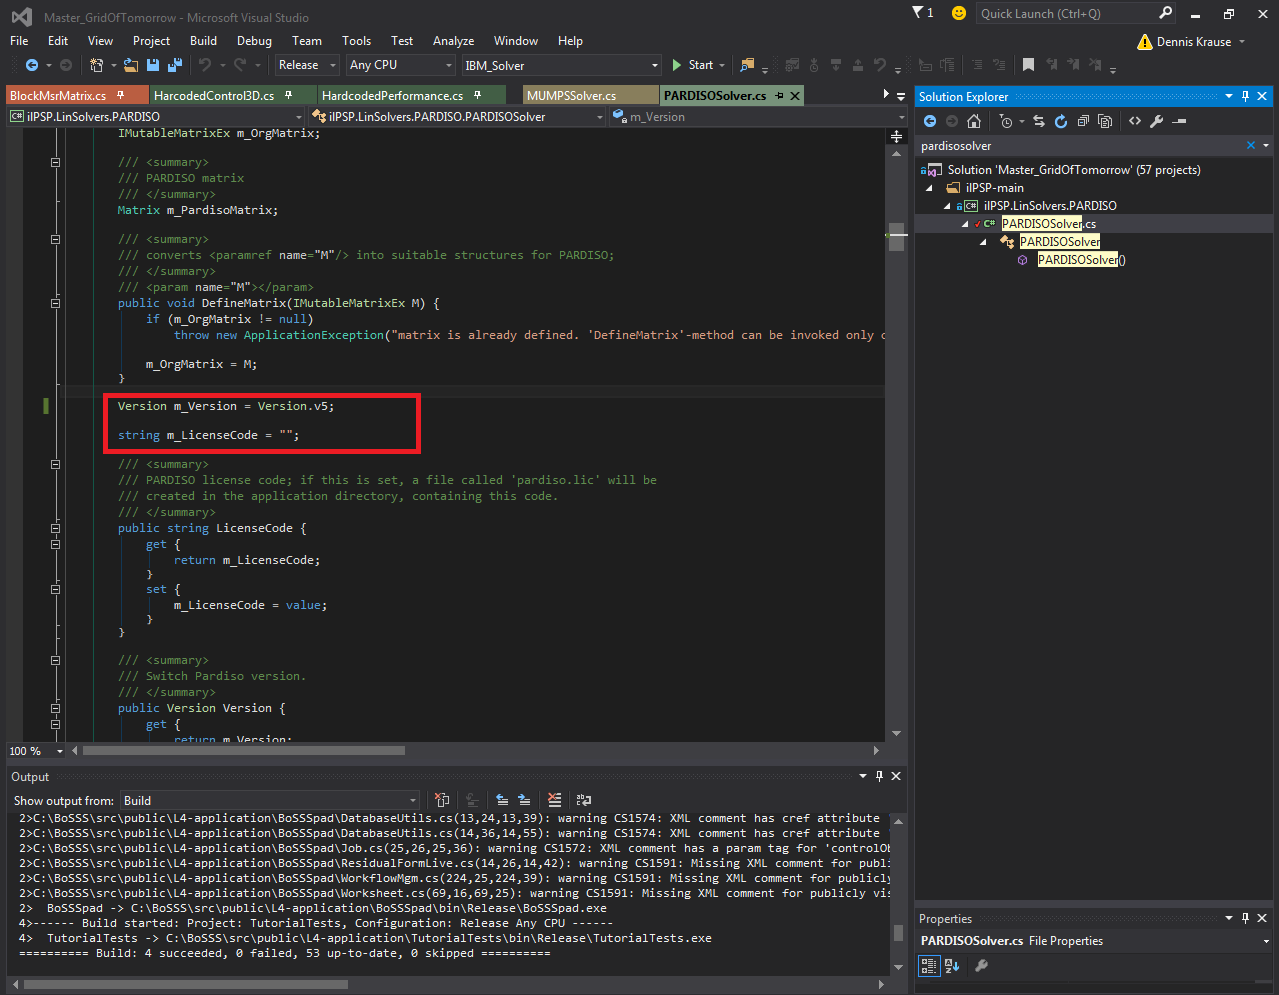
\includegraphics[width=\textwidth]{Figures/bossspad_pardiso.png}\\
	\end{centering}
	\caption{Inserting your own \emph{PARDISO} license key for using \emph{BoSSSpad} on the Lichtenberg cluster. Use this version for the Lichtenberg cluster.}\label{fig:pardiso_bossspad}
\end{figure} %


Obviously, the list of databases will be empty on the first start, since the location of the databases on the cluster has not been configured yet. In order to do so, you have to create a database configuration file at \verb|~/.BoSSS/etc/DBE.xml| by hand. The content of the file should be given by

\begin{minipage}{\linewidth}
\begin{lstlisting}
<?xml version="1.0" encoding="utf-8"?>
<DBEControl>
  <Databases>
    <Database>
      <path value="/home/$TuID/bosss_db" />
    </Database>
  </Databases>
</DBEControl>
\end{lstlisting}
\end{minipage}

if your database is located at \verb|~/bosss_db|. When you start the \emph{BoSSSpad} the next time, this database should be loaded automatically.

\begin{figure}[htbp]
	\begin{centering}
		\subfloat[Checkbox]{
			\label{fig:puttyXFowarding_checkbox}
			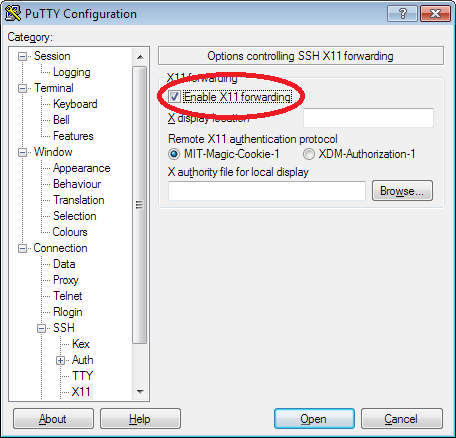
\includegraphics[height=0.25\textheight]{Figures/puttyXForwarding.png}}
		\qquad
		\subfloat[Exemplary output]{
			\label{fig:puttyXFowarding_output}
			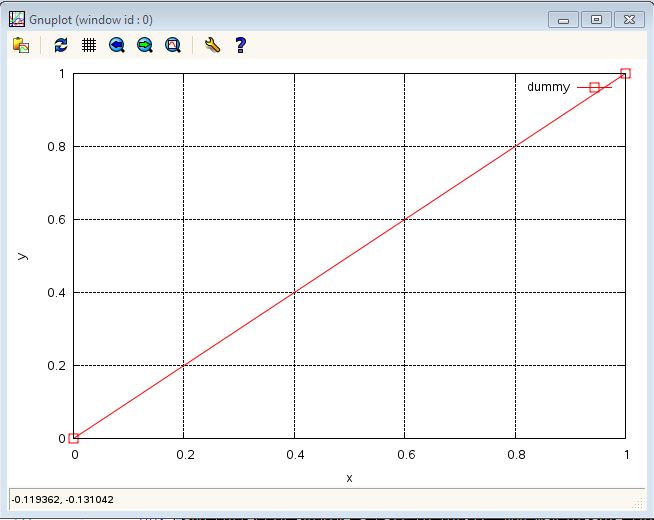
\includegraphics[height=0.25\textheight]{Figures/gnuplot.png}}
	\end{centering}
	\caption{PuTTY - Forwarding of graphical output}
	\label{fig:puttyXFowarding}
\end{figure}

Some parts of the \emph{BoSSSpad} create graphical output (e.g., when plotting the residuals). In order to be able to use this feature on the cluster, you to forward graphical output to your local machine. This feature is called \emph{X11} forwarding and is activated by establishing the connection via
\begin{verbatim}
ssh -X $TuID@$host
\end{verbatim}
or by checking the corresponding in \emph{PuTTY} (see Figure \ref{fig:puttyXFowarding_checkbox}). Moreover, you need a software that is able to render the graphical output from the cluster on your local machine. To that end, you have to make sure that the tool \emph{Xming} is running when connecting to the cluster. The tool should already be installed on all machines at the fdy. After starting, it automatically minimizes to the system tray and waits for input to render.

You can test your setup by starting the \emph{BoSSSpad} on the cluster and running the command
\begin{verbatim}
new DataSet(new double[] { 0, 1 }, new double[] { 0, 1 }, "dummy").Plot()
\end{verbatim}
which should generate the graph displayed in Figure \ref{fig:puttyXFowarding_output} on your local machine.
\subsubsection{Troubleshooting}
\begin{itemize}
\item \textbf{MPI-Error}:  The \emph{BoSSSpad} uses MPI communication, hence the MPI module needs to be loaded before starting the \emph{BoSSSpad} via
\begin{verbatim}
module load openmpi/gcc/1.6.6
\end{verbatim}
\item \textbf{Library missing}: After deploying the \emph{BoSSSpad}, the BoSSSpad folder contains a file \emph{Mono.CSharp.dll}. It can be that the \emph{BoSSSpad} doesn't find this library, because it searches for \emph{Mono.Csharp.dll}. Just copy the file:
\begin{verbatim}
cp Mono.CSharp.dll Mono.Csharp.dll
\end{verbatim}
\item The \textbf{git-bash} on windows machines causes some problems after starting the \emph{BoSSSpad}, i.e. only a black display appears and the program crashes. So far only the \emph{BoSSSpad} only runs with \emph{PuTTY}.
\end{itemize}


%==================== Literatur =====================================
% Bibliography
% -------------
%\bibliography{BibDaten}

%==================== Anhang ========================================
%\appendix

\clearemptydoublepage

\end{document}
